\documentclass[11pt,preprint, authoryear]{elsarticle}

\usepackage{lmodern}
%%%% My spacing
\usepackage{setspace}
\setstretch{1.2}
\DeclareMathSizes{12}{14}{10}{10}

% Wrap around which gives all figures included the [H] command, or places it "here". This can be tedious to code in Rmarkdown.
\usepackage{float}
\let\origfigure\figure
\let\endorigfigure\endfigure
\renewenvironment{figure}[1][2] {
    \expandafter\origfigure\expandafter[H]
} {
    \endorigfigure
}

\let\origtable\table
\let\endorigtable\endtable
\renewenvironment{table}[1][2] {
    \expandafter\origtable\expandafter[H]
} {
    \endorigtable
}


\usepackage{ifxetex,ifluatex}
\usepackage{fixltx2e} % provides \textsubscript
\ifnum 0\ifxetex 1\fi\ifluatex 1\fi=0 % if pdftex
  \usepackage[T1]{fontenc}
  \usepackage[utf8]{inputenc}
\else % if luatex or xelatex
  \ifxetex
    \usepackage{mathspec}
    \usepackage{xltxtra,xunicode}
  \else
    \usepackage{fontspec}
  \fi
  \defaultfontfeatures{Mapping=tex-text,Scale=MatchLowercase}
  \newcommand{\euro}{€}
\fi

\usepackage{amssymb, amsmath, amsthm, amsfonts}

\def\bibsection{\section*{References}} %%% Make "References" appear before bibliography


\usepackage[round]{natbib}

\usepackage{longtable}
\usepackage[margin=2.3cm,bottom=2cm,top=2.5cm, includefoot]{geometry}
\usepackage{fancyhdr}
\usepackage[bottom, hang, flushmargin]{footmisc}
\usepackage{graphicx}
\numberwithin{equation}{section}
\numberwithin{figure}{section}
\numberwithin{table}{section}
\setlength{\parindent}{0cm}
\setlength{\parskip}{1.3ex plus 0.5ex minus 0.3ex}
\usepackage{textcomp}
\renewcommand{\headrulewidth}{0.2pt}
\renewcommand{\footrulewidth}{0.3pt}

\usepackage{array}
\newcolumntype{x}[1]{>{\centering\arraybackslash\hspace{0pt}}p{#1}}

%%%%  Remove the "preprint submitted to" part. Don't worry about this either, it just looks better without it:
\makeatletter
\def\ps@pprintTitle{%
  \let\@oddhead\@empty
  \let\@evenhead\@empty
  \let\@oddfoot\@empty
  \let\@evenfoot\@oddfoot
}
\makeatother

 \def\tightlist{} % This allows for subbullets!

\usepackage{hyperref}
\hypersetup{breaklinks=true,
            bookmarks=true,
            colorlinks=true,
            citecolor=blue,
            urlcolor=blue,
            linkcolor=blue,
            pdfborder={0 0 0}}


% The following packages allow huxtable to work:
\usepackage{siunitx}
\usepackage{multirow}
\usepackage{hhline}
\usepackage{calc}
\usepackage{tabularx}
\usepackage{booktabs}
\usepackage{caption}


\newenvironment{columns}[1][]{}{}

\newenvironment{column}[1]{\begin{minipage}{#1}\ignorespaces}{%
\end{minipage}
\ifhmode\unskip\fi
\aftergroup\useignorespacesandallpars}

\def\useignorespacesandallpars#1\ignorespaces\fi{%
#1\fi\ignorespacesandallpars}

\makeatletter
\def\ignorespacesandallpars{%
  \@ifnextchar\par
    {\expandafter\ignorespacesandallpars\@gobble}%
    {}%
}
\makeatother

\newlength{\cslhangindent}
\setlength{\cslhangindent}{1.5em}
\newenvironment{CSLReferences}%
  {\setlength{\parindent}{0pt}%
  \everypar{\setlength{\hangindent}{\cslhangindent}}\ignorespaces}%
  {\par}


\urlstyle{same}  % don't use monospace font for urls
\setlength{\parindent}{0pt}
\setlength{\parskip}{6pt plus 2pt minus 1pt}
\setlength{\emergencystretch}{3em}  % prevent overfull lines
\setcounter{secnumdepth}{5}

%%% Use protect on footnotes to avoid problems with footnotes in titles
\let\rmarkdownfootnote\footnote%
\def\footnote{\protect\rmarkdownfootnote}
\IfFileExists{upquote.sty}{\usepackage{upquote}}{}

%%% Include extra packages specified by user
\usepackage{booktabs}
\usepackage{longtable}
\usepackage{array}
\usepackage{multirow}
\usepackage{wrapfig}
\usepackage{float}
\usepackage{colortbl}
\usepackage{pdflscape}
\usepackage{tabu}
\usepackage{threeparttable}
\usepackage{threeparttablex}
\usepackage[normalem]{ulem}
\usepackage{makecell}
\usepackage{xcolor}
\usepackage{caption}
\usepackage{graphicx}
\usepackage{siunitx}
\usepackage{hhline}
\usepackage{calc}
\usepackage{tabularx}
\usepackage{adjustbox}
\usepackage{hyperref}

%%% Hard setting column skips for reports - this ensures greater consistency and control over the length settings in the document.
%% page layout
%% paragraphs
\setlength{\baselineskip}{12pt plus 0pt minus 0pt}
\setlength{\parskip}{12pt plus 0pt minus 0pt}
\setlength{\parindent}{0pt plus 0pt minus 0pt}
%% floats
\setlength{\floatsep}{12pt plus 0 pt minus 0pt}
\setlength{\textfloatsep}{20pt plus 0pt minus 0pt}
\setlength{\intextsep}{14pt plus 0pt minus 0pt}
\setlength{\dbltextfloatsep}{20pt plus 0pt minus 0pt}
\setlength{\dblfloatsep}{14pt plus 0pt minus 0pt}
%% maths
\setlength{\abovedisplayskip}{12pt plus 0pt minus 0pt}
\setlength{\belowdisplayskip}{12pt plus 0pt minus 0pt}
%% lists
\setlength{\topsep}{10pt plus 0pt minus 0pt}
\setlength{\partopsep}{3pt plus 0pt minus 0pt}
\setlength{\itemsep}{5pt plus 0pt minus 0pt}
\setlength{\labelsep}{8mm plus 0mm minus 0mm}
\setlength{\parsep}{\the\parskip}
\setlength{\listparindent}{\the\parindent}
%% verbatim
\setlength{\fboxsep}{5pt plus 0pt minus 0pt}


\usepackage{color}
\usepackage{fancyvrb}
\newcommand{\VerbBar}{|}
\newcommand{\VERB}{\Verb[commandchars=\\\{\}]}
\DefineVerbatimEnvironment{Highlighting}{Verbatim}{commandchars=\\\{\}}
% Add ',fontsize=\small' for more characters per line
\usepackage{framed}
\definecolor{shadecolor}{RGB}{248,248,248}
\newenvironment{Shaded}{\begin{snugshade}}{\end{snugshade}}
\newcommand{\AlertTok}[1]{\textcolor[rgb]{0.94,0.16,0.16}{#1}}
\newcommand{\AnnotationTok}[1]{\textcolor[rgb]{0.56,0.35,0.01}{\textbf{\textit{#1}}}}
\newcommand{\AttributeTok}[1]{\textcolor[rgb]{0.77,0.63,0.00}{#1}}
\newcommand{\BaseNTok}[1]{\textcolor[rgb]{0.00,0.00,0.81}{#1}}
\newcommand{\BuiltInTok}[1]{#1}
\newcommand{\CharTok}[1]{\textcolor[rgb]{0.31,0.60,0.02}{#1}}
\newcommand{\CommentTok}[1]{\textcolor[rgb]{0.56,0.35,0.01}{\textit{#1}}}
\newcommand{\CommentVarTok}[1]{\textcolor[rgb]{0.56,0.35,0.01}{\textbf{\textit{#1}}}}
\newcommand{\ConstantTok}[1]{\textcolor[rgb]{0.00,0.00,0.00}{#1}}
\newcommand{\ControlFlowTok}[1]{\textcolor[rgb]{0.13,0.29,0.53}{\textbf{#1}}}
\newcommand{\DataTypeTok}[1]{\textcolor[rgb]{0.13,0.29,0.53}{#1}}
\newcommand{\DecValTok}[1]{\textcolor[rgb]{0.00,0.00,0.81}{#1}}
\newcommand{\DocumentationTok}[1]{\textcolor[rgb]{0.56,0.35,0.01}{\textbf{\textit{#1}}}}
\newcommand{\ErrorTok}[1]{\textcolor[rgb]{0.64,0.00,0.00}{\textbf{#1}}}
\newcommand{\ExtensionTok}[1]{#1}
\newcommand{\FloatTok}[1]{\textcolor[rgb]{0.00,0.00,0.81}{#1}}
\newcommand{\FunctionTok}[1]{\textcolor[rgb]{0.00,0.00,0.00}{#1}}
\newcommand{\ImportTok}[1]{#1}
\newcommand{\InformationTok}[1]{\textcolor[rgb]{0.56,0.35,0.01}{\textbf{\textit{#1}}}}
\newcommand{\KeywordTok}[1]{\textcolor[rgb]{0.13,0.29,0.53}{\textbf{#1}}}
\newcommand{\NormalTok}[1]{#1}
\newcommand{\OperatorTok}[1]{\textcolor[rgb]{0.81,0.36,0.00}{\textbf{#1}}}
\newcommand{\OtherTok}[1]{\textcolor[rgb]{0.56,0.35,0.01}{#1}}
\newcommand{\PreprocessorTok}[1]{\textcolor[rgb]{0.56,0.35,0.01}{\textit{#1}}}
\newcommand{\RegionMarkerTok}[1]{#1}
\newcommand{\SpecialCharTok}[1]{\textcolor[rgb]{0.00,0.00,0.00}{#1}}
\newcommand{\SpecialStringTok}[1]{\textcolor[rgb]{0.31,0.60,0.02}{#1}}
\newcommand{\StringTok}[1]{\textcolor[rgb]{0.31,0.60,0.02}{#1}}
\newcommand{\VariableTok}[1]{\textcolor[rgb]{0.00,0.00,0.00}{#1}}
\newcommand{\VerbatimStringTok}[1]{\textcolor[rgb]{0.31,0.60,0.02}{#1}}
\newcommand{\WarningTok}[1]{\textcolor[rgb]{0.56,0.35,0.01}{\textbf{\textit{#1}}}}

\begin{document}



\begin{frontmatter}  %

\title{Exploring Machine Learning and Predicting Income}

% Set to FALSE if wanting to remove title (for submission)




\author[Add1]{Cassandra Pengelly}
\ead{20346212@sun.ac.za}








\vspace{1cm}





\vspace{0.5cm}

\end{frontmatter}



%________________________
% Header and Footers
%%%%%%%%%%%%%%%%%%%%%%%%%%%%%%%%%
\pagestyle{fancy}
\chead{}
\rhead{}
\lfoot{}
\rfoot{\footnotesize Page \thepage}
\lhead{}
%\rfoot{\footnotesize Page \thepage } % "e.g. Page 2"
\cfoot{}

%\setlength\headheight{30pt}
%%%%%%%%%%%%%%%%%%%%%%%%%%%%%%%%%
%________________________

\headsep 35pt % So that header does not go over title




\hypertarget{introduction}{%
\section{\texorpdfstring{Introduction
\label{Introduction}}{Introduction }}\label{introduction}}

Labour economists have long been interested in the identifying the
factors that influence a person's income.

This paper investigates how well machine learning techniques can predict
income and race. The focus is on machine learning and the code, rather
than the economic interpretation of the model results.

This paper\footnote{This assignment was written using the package by
  \protect\hyperlink{ref-Texevier}{Katzke}
  (\protect\hyperlink{ref-Texevier}{2017})} is structured as follows.
First, the data set - NIDS - is discussed in section \ref{Data}; then
the methodology is explained in section \ref{Meth}. Section \ref{ML}
applies machine learning techniques to the NIDS data set, and comprises
two subsections. The first subsection (\ref{income}) compares the
effectiveness of linear regression and regularised regression on
predicting people's incomes. The second subsection (\ref{race})
evaluated 5 classification algrithms - Linear Discriminant Analysis,
Classification and Regression Trees, k-Nearest Neighbors, Support Vector
Machines with a linear kernel and Random Forest - on their accuracy in
predicting a person's race.

\hypertarget{data}{%
\section{\texorpdfstring{Data \label{Data}}{Data }}\label{data}}

The data used for this assignment was sourced from Wave 5 of the
National Income Dynamics Survey (NIDS)
(\protect\hyperlink{ref-nids}{\emph{National income dynamics study 2017,
wave 5 dataset}} (\protect\hyperlink{ref-nids}{2018})). The survey is a
nationally representative household panel study, which started in 2008
with a group of over 28,000 individuals from 7,300 households. The same
households are surveyed every 2 years for NIDS. The latest survey - wave
5 - was conducted in 2017. For wave 5, a total of 39,434 individuals
were interviewed; 20,113 of which were part of the original study - wave
1 - and 2,016 were from a top-up sample. NIDS is funded by the
Department of Planning, Monitoring and Evaluation and the survey is
implemented by the Southern Africa Labour and Development Research Unit
(SALDRU) at the University of Cape Town. The data set is comprehensive
and covers topics relating to poverty, health, household composition,
mortality, expenditure, income and employment. The NIDS data set is
partitioned into different units of observations (e.g.~adults, children,
household etc.); for this assignment, data on adults was used.

One weakness of the NIDS data set is that it suffers from the common
problem that households at the higher end of the income distribution
tend to be underrepresented. This could be explained by the fact that
the rich refuse to fill out forms or they underreport their incomes.
Because race and income are highly correlated in South Africa, this
could also imply that white people are undersampled. To correct for the
sample data not representing the population income/race distribution,
some balancing techniques are applied in section \ref{race}.

\hypertarget{methodology}{%
\section{\texorpdfstring{Methodology
\label{Meth}}{Methodology }}\label{methodology}}

I first made use of SQLite\footnote{I found I struggle quite a bit using
  SQL but it has got easier with practice. I'm still not 100\%
  comfortable with it so I used dplyr to manipulate the data for the
  machine learning section.} to investigate and visualise the data. I
first ran the code in the R script called SQL. I opened a new connection
and called it nids, and wrote the NIDS data, which included waves 2-5,
into tables in the NIDS database. I used a few lines of code to check
what tables were in nids and what their source was. Then I started to
explore the NIDS wave 5 data, for example looking at the column names. I
queried the data and selected 7 variables for analysis: date of birth,
income, gender, marital status, race, years of schooling and tertiary
qualification. I used date of birth to calculate the variable `age'.

I cleaned the data by renaming the variables to be reader-friendly and
removed values that were nonsensical (e.g.~negative years of schooling)
by applying filters to the data. I wanted to see the proportion of the
races so I first manipulated the data in the SQL script and then used
the function `show\_query' to get the code for SQL. I copied this into
the r chunk in the markdown file and then graphed the results using
ggplot2. The code below shows some of this process and output:

\begin{Shaded}
\begin{Highlighting}[]
\FunctionTok{library}\NormalTok{(DBI)}
\NormalTok{nids }\OtherTok{\textless{}{-}}\NormalTok{ DBI}\SpecialCharTok{::}\FunctionTok{dbConnect}\NormalTok{(RSQLite}\SpecialCharTok{::}\FunctionTok{SQLite}\NormalTok{(), }\StringTok{"data/nids{-}db\textasciitilde{}output.sqlite"}\NormalTok{)}
\end{Highlighting}
\end{Shaded}

\begin{Shaded}
\begin{Highlighting}[]
\KeywordTok{SELECT}\NormalTok{ \textasciigrave{}race\textasciigrave{}, }\FunctionTok{COUNT}\NormalTok{(}\OperatorTok{*}\NormalTok{) }\KeywordTok{AS}\NormalTok{ \textasciigrave{}n\textasciigrave{}}
\KeywordTok{FROM}\NormalTok{ (}\KeywordTok{SELECT}\NormalTok{ \textasciigrave{}w5\_a\_dob\_y\textasciigrave{}, \textasciigrave{}w5\_a\_gen\textasciigrave{} }\KeywordTok{AS}\NormalTok{ \textasciigrave{}gender\textasciigrave{}, \textasciigrave{}w5\_a\_popgrp\textasciigrave{} }\KeywordTok{AS}\NormalTok{ \textasciigrave{}race\textasciigrave{}, }
\NormalTok{\textasciigrave{}w5\_a\_em1pay\textasciigrave{} }\KeywordTok{AS}\NormalTok{ \textasciigrave{}income\textasciigrave{}, \textasciigrave{}w5\_a\_mar\textasciigrave{} }\KeywordTok{AS}\NormalTok{ \textasciigrave{}married\textasciigrave{}, \textasciigrave{}w5\_a\_edschgrd\textasciigrave{} }\KeywordTok{AS}\NormalTok{ \textasciigrave{}school\textasciigrave{}, }
\NormalTok{\textasciigrave{}w5\_a\_edter\textasciigrave{} }\KeywordTok{AS}\NormalTok{ \textasciigrave{}tertiary\textasciigrave{} }\KeywordTok{FROM}\NormalTok{ \textasciigrave{}wave5\textasciigrave{}) }\KeywordTok{WHERE}\NormalTok{ (\textasciigrave{}race\textasciigrave{} }\OperatorTok{\textgreater{}} \FloatTok{0.0} \KeywordTok{AND}\NormalTok{ \textasciigrave{}race\textasciigrave{} }\OperatorTok{\textless{}} \FloatTok{5.0}\NormalTok{)}
\KeywordTok{GROUP} \KeywordTok{BY}\NormalTok{ \textasciigrave{}race\textasciigrave{}}
\end{Highlighting}
\end{Shaded}

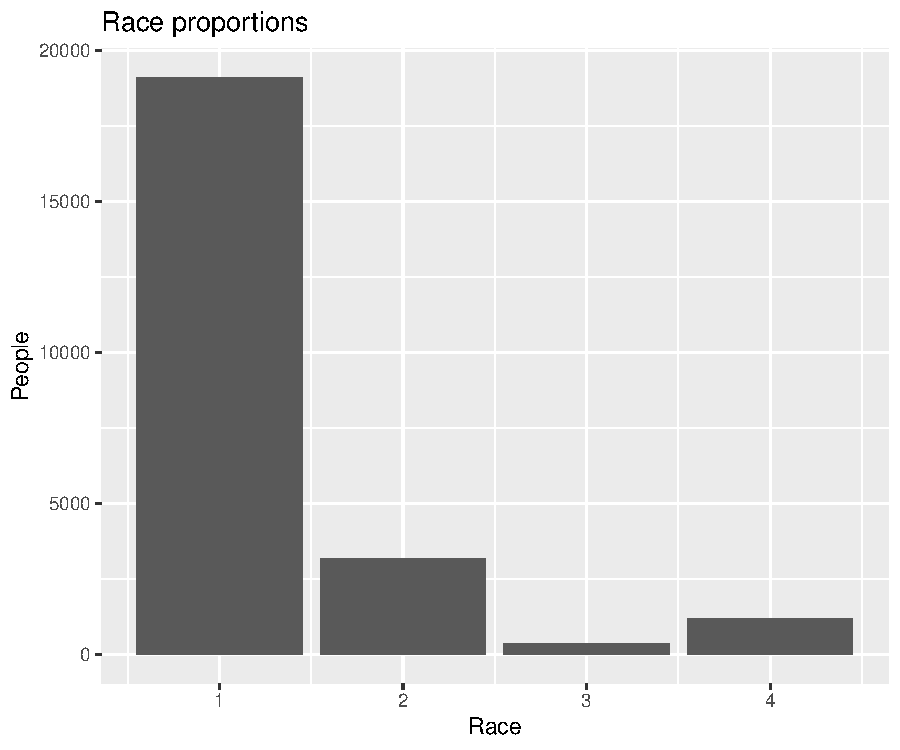
\includegraphics{20346212MLProject_files/figure-latex/unnamed-chunk-3-1.pdf}

\begin{tabular}{l}
\hline
Race\\
\hline
1 = African\\
\hline
2 = Coloured\\
\hline
3 = Asian/Indian\\
\hline
4 = White\\
\hline
\end{tabular}

The bar graph above shows that the majority of people sampled are
African and the smallest proportion are Asian/Indian. In general the
proportions appear to match the race distribution of South Africans. The
histogram below reports the number of years of schooling. We can see
that the majority of the sample has had 12 years of schooling. The data
for this graph was also manipulated using the SQL script and then the
SQL code was copied into the r chunk.

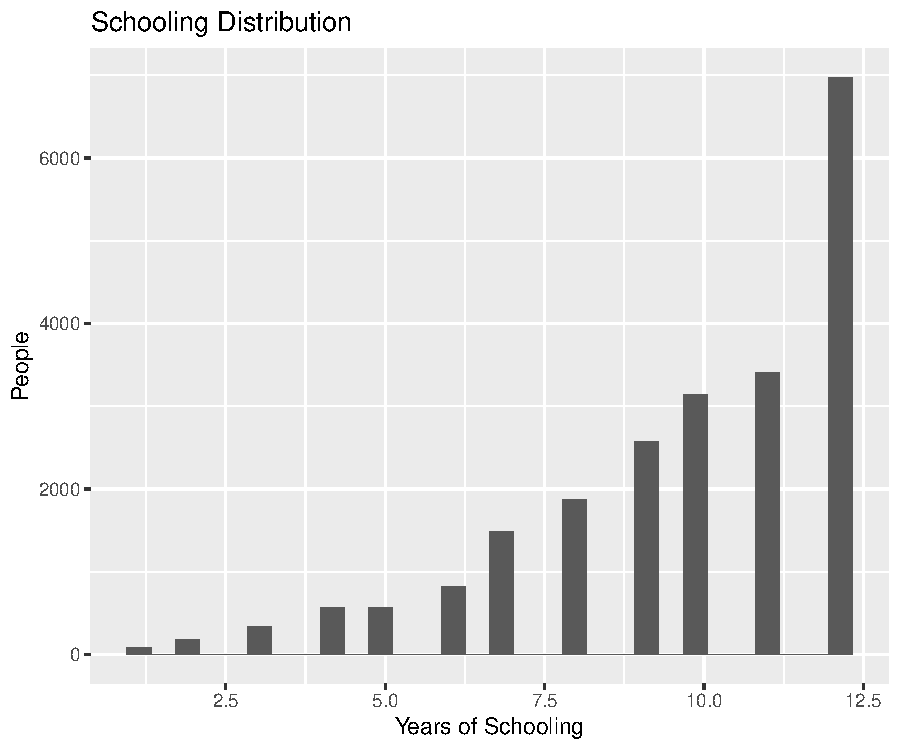
\includegraphics{20346212MLProject_files/figure-latex/unnamed-chunk-5-1.pdf}

Looking at the proportion of people who are married versus those that
are not, we can clearly see that there are more people married than
unmarried in this sample, as the bar graph below demonstrates.

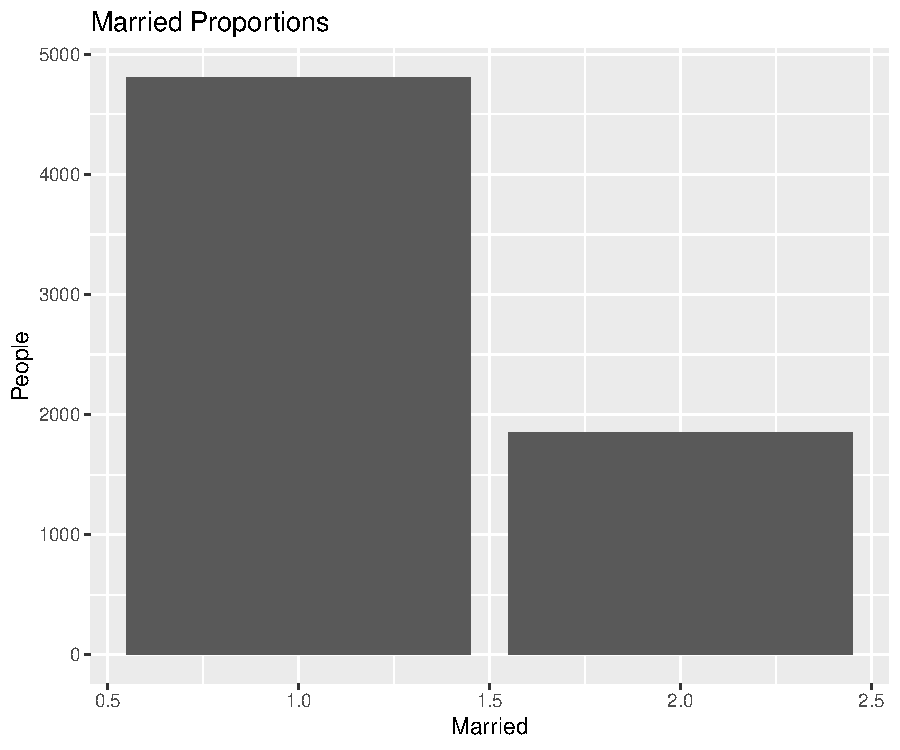
\includegraphics{20346212MLProject_files/figure-latex/unnamed-chunk-7-1.pdf}

\begin{tabular}{l}
\hline
Married\\
\hline
1 = Married\\
\hline
2 = Not married\\
\hline
\end{tabular}

If I had wanted to use more than one of the NIDS data sets, say wave 4
and 5, I could merge the two data sets using the SQL code below. I
lightly cleaned both data sets beforehand and then used the union\_all
function to merge them.

\begin{Shaded}
\begin{Highlighting}[]
\KeywordTok{SELECT} \FloatTok{2021.0} \OperatorTok{{-}}\NormalTok{ \textasciigrave{}w5\_a\_dob\_y\textasciigrave{} }\KeywordTok{AS}\NormalTok{ \textasciigrave{}age\textasciigrave{}, \textasciigrave{}w5\_a\_gen\textasciigrave{} }\KeywordTok{AS}\NormalTok{ \textasciigrave{}gender\textasciigrave{}, \textasciigrave{}w5\_a\_popgrp\textasciigrave{} }\KeywordTok{AS}\NormalTok{ \textasciigrave{}race\textasciigrave{}, }
\NormalTok{\textasciigrave{}w5\_a\_em1pay\textasciigrave{} }\KeywordTok{AS}\NormalTok{ \textasciigrave{}income\textasciigrave{}, \textasciigrave{}w5\_a\_mar\textasciigrave{} }\KeywordTok{AS}\NormalTok{ \textasciigrave{}married\textasciigrave{}, \textasciigrave{}w5\_a\_edschgrd\textasciigrave{} }\KeywordTok{AS}\NormalTok{ \textasciigrave{}school\textasciigrave{}, }
\NormalTok{\textasciigrave{}w5\_a\_edter\textasciigrave{} }\KeywordTok{AS}\NormalTok{ \textasciigrave{}tertiary\textasciigrave{} }\KeywordTok{FROM}\NormalTok{ \textasciigrave{}wave5\textasciigrave{}}
\KeywordTok{UNION} \KeywordTok{ALL}
\KeywordTok{SELECT} \FloatTok{2021.0} \OperatorTok{{-}}\NormalTok{ \textasciigrave{}w4\_a\_dob\_y\textasciigrave{} }\KeywordTok{AS}\NormalTok{ \textasciigrave{}age\textasciigrave{}, \textasciigrave{}w4\_a\_gen\textasciigrave{} }\KeywordTok{AS}\NormalTok{ \textasciigrave{}gender\textasciigrave{}, \textasciigrave{}w4\_a\_popgrp\textasciigrave{} }\KeywordTok{AS}\NormalTok{ \textasciigrave{}race\textasciigrave{}, }
\NormalTok{\textasciigrave{}w4\_a\_em1pay\textasciigrave{} }\KeywordTok{AS}\NormalTok{ \textasciigrave{}income\textasciigrave{}, \textasciigrave{}w4\_a\_mar\textasciigrave{} }\KeywordTok{AS}\NormalTok{ \textasciigrave{}married\textasciigrave{}, \textasciigrave{}w4\_a\_edschgrd\textasciigrave{} }\KeywordTok{AS}\NormalTok{ \textasciigrave{}school\textasciigrave{}, }
\NormalTok{\textasciigrave{}w4\_a\_edter\textasciigrave{} }\KeywordTok{AS}\NormalTok{ \textasciigrave{}tertiary\textasciigrave{} }\KeywordTok{FROM}\NormalTok{ \textasciigrave{}wave4\textasciigrave{}}
\end{Highlighting}
\end{Shaded}

The table below provides a glimpse into the first 5 rows of the newly
joined data set. I output a variable in the previous chunk as a
dataframe and then displayed the dataframe in a table in the next r
chunk. However, I could have used the function `head' in the SQL script
on the joined dataframe and the used the `collect()' function to save
the output to a global object and then displayed that object as a
dataframe.

\begin{tabular}{r|r|r|r|r|r|r}
\hline
age & gender & race & income & married & school & tertiary\\
\hline
41 & 1 & 2 & 23752 & 1 & 12 & 1\\
\hline
28 & 1 & 1 & NA & NA & 10 & 2\\
\hline
42 & 2 & 1 & NA & 1 & 11 & 1\\
\hline
49 & 1 & 1 & NA & 1 & 11 & 1\\
\hline
54 & 1 & 1 & NA & NA & 25 & NA\\
\hline
\end{tabular}

After the initial data exploration I decided to focus on predicting
income and race using machine learning techniques, which are presented
in the following section.

\hypertarget{machine-learning}{%
\section{\texorpdfstring{Machine Learning
\label{ML}}{Machine Learning }}\label{machine-learning}}

\hypertarget{predicting-income}{%
\subsection{\texorpdfstring{Predicting Income
\label{income}}{Predicting Income }}\label{predicting-income}}

Econometrics often makes use of regression analysis to model economic
phenomena, test economic hypotheses and to forecast economic activity
\protect\hyperlink{ref-econ}{Studenmund}
(\protect\hyperlink{ref-econ}{2014: 2}). A popular method in econometric
regression modeling is that of Ordinary Least Squares; however, advances
in machine learning have presented alternative/augmenting methods that
may be (more) useful. One such augmenting method is K-fold cross
validation, which evaluates the skill of machine learning models. As
\protect\hyperlink{ref-kfold}{Rodriguez, Perez \& Lozano}
(\protect\hyperlink{ref-kfold}{2009: 569}) explain, in K-fold cross
validation, a data set is randomly split into \(k\) number of groups, of
similar sizes. The first group is considered a validation set and the
method is fitted to the other \(k-1\) groups.

Below, \ref{Regression} displays 3 different linear regressions of log
of income using K-fold cross validation. For these regressions I built a
function ``linreg'', which takes in a data frame, cleans and splits the
data into a training (70\% of the full data set) and a test set (30\% of
the full data set) and runs 3 different linear regressions, applying
K-fold cross validation. The sample size for regressions amounts to 4258
observations, with the training and testing sets amounting to 2982 and
1276 respectively. The results of the regressions are then collected and
stored in a list, which is returned by the function. I use k = 10,
because empirically k=10 has been shown have test error rate estimates
that have relatively low bias and variance
(\protect\hyperlink{ref-k}{Kassambara}
(\protect\hyperlink{ref-k}{2018a})). I have also set seed in the
function for reproducibility.

Based on the Mincerian wage equation, Regression 1 (see
\ref{Regression}) regresses log of income on age, years of schooling and
a dummy variable for if a person has a tertiary qualification or not.
Regression 2 includes a variable for age-squared and the categorical
variable race. Regression 3 includes a variable each for gender and
marriage. The signs of the coefficients of the three regressions look
fairly standard\footnote{This at least is a good indication that the
  data is fairly well cleaned and is usable for testing the machine
  learning techniques} and most of the coefficients are statistically
significant at 1\% and lower. For the variables whose coefficients are
not statistically significant, labour market literature and economic
theory suggest that they are important controls and should be included,
which justifies their presence.

 
  \providecommand{\huxb}[2]{\arrayrulecolor[RGB]{#1}\global\arrayrulewidth=#2pt}
  \providecommand{\huxvb}[2]{\color[RGB]{#1}\vrule width #2pt}
  \providecommand{\huxtpad}[1]{\rule{0pt}{#1}}
  \providecommand{\huxbpad}[1]{\rule[-#1]{0pt}{#1}}

\begin{table}[ht]
\begin{centerbox}
\begin{threeparttable}
\captionsetup{justification=centering,singlelinecheck=off}
\caption{Log-Income Regression Output}
 \label{Regression}
\setlength{\tabcolsep}{0pt}
\begin{tabular}{l l l l}


\hhline{>{\huxb{0, 0, 0}{0.8}}->{\huxb{0, 0, 0}{0.8}}->{\huxb{0, 0, 0}{0.8}}->{\huxb{0, 0, 0}{0.8}}-}
\arrayrulecolor{black}

\multicolumn{1}{!{\huxvb{0, 0, 0}{0}}c!{\huxvb{0, 0, 0}{0}}}{\huxtpad{6pt + 1em}\centering \hspace{6pt} {\fontsize{12pt}{14.4pt}\selectfont } \hspace{6pt}\huxbpad{6pt}} &
\multicolumn{1}{c!{\huxvb{0, 0, 0}{0}}}{\huxtpad{6pt + 1em}\centering \hspace{6pt} {\fontsize{12pt}{14.4pt}\selectfont Reg 1} \hspace{6pt}\huxbpad{6pt}} &
\multicolumn{1}{c!{\huxvb{0, 0, 0}{0}}}{\huxtpad{6pt + 1em}\centering \hspace{6pt} {\fontsize{12pt}{14.4pt}\selectfont Reg 2} \hspace{6pt}\huxbpad{6pt}} &
\multicolumn{1}{c!{\huxvb{0, 0, 0}{0}}}{\huxtpad{6pt + 1em}\centering \hspace{6pt} {\fontsize{12pt}{14.4pt}\selectfont Reg 3} \hspace{6pt}\huxbpad{6pt}} \tabularnewline[-0.5pt]


\hhline{>{\huxb{255, 255, 255}{0.4}}->{\huxb{0, 0, 0}{0.4}}->{\huxb{0, 0, 0}{0.4}}->{\huxb{0, 0, 0}{0.4}}-}
\arrayrulecolor{black}

\multicolumn{1}{!{\huxvb{0, 0, 0}{0}}l!{\huxvb{0, 0, 0}{0}}}{\huxtpad{6pt + 1em}\raggedright \hspace{6pt} {\fontsize{12pt}{14.4pt}\selectfont (Intercept)} \hspace{6pt}\huxbpad{6pt}} &
\multicolumn{1}{r!{\huxvb{0, 0, 0}{0}}}{\huxtpad{6pt + 1em}\raggedleft \hspace{6pt} {\fontsize{12pt}{14.4pt}\selectfont 6.097 ***} \hspace{6pt}\huxbpad{6pt}} &
\multicolumn{1}{r!{\huxvb{0, 0, 0}{0}}}{\huxtpad{6pt + 1em}\raggedleft \hspace{6pt} {\fontsize{12pt}{14.4pt}\selectfont 5.791 ***} \hspace{6pt}\huxbpad{6pt}} &
\multicolumn{1}{r!{\huxvb{0, 0, 0}{0}}}{\huxtpad{6pt + 1em}\raggedleft \hspace{6pt} {\fontsize{12pt}{14.4pt}\selectfont 5.526 ***} \hspace{6pt}\huxbpad{6pt}} \tabularnewline[-0.5pt]


\hhline{}
\arrayrulecolor{black}

\multicolumn{1}{!{\huxvb{0, 0, 0}{0}}l!{\huxvb{0, 0, 0}{0}}}{\huxtpad{6pt + 1em}\raggedright \hspace{6pt} {\fontsize{12pt}{14.4pt}\selectfont } \hspace{6pt}\huxbpad{6pt}} &
\multicolumn{1}{r!{\huxvb{0, 0, 0}{0}}}{\huxtpad{6pt + 1em}\raggedleft \hspace{6pt} {\fontsize{12pt}{14.4pt}\selectfont (0.145)~~~} \hspace{6pt}\huxbpad{6pt}} &
\multicolumn{1}{r!{\huxvb{0, 0, 0}{0}}}{\huxtpad{6pt + 1em}\raggedleft \hspace{6pt} {\fontsize{12pt}{14.4pt}\selectfont (0.367)~~~} \hspace{6pt}\huxbpad{6pt}} &
\multicolumn{1}{r!{\huxvb{0, 0, 0}{0}}}{\huxtpad{6pt + 1em}\raggedleft \hspace{6pt} {\fontsize{12pt}{14.4pt}\selectfont (0.354)~~~} \hspace{6pt}\huxbpad{6pt}} \tabularnewline[-0.5pt]


\hhline{}
\arrayrulecolor{black}

\multicolumn{1}{!{\huxvb{0, 0, 0}{0}}l!{\huxvb{0, 0, 0}{0}}}{\huxtpad{6pt + 1em}\raggedright \hspace{6pt} {\fontsize{12pt}{14.4pt}\selectfont age} \hspace{6pt}\huxbpad{6pt}} &
\multicolumn{1}{r!{\huxvb{0, 0, 0}{0}}}{\huxtpad{6pt + 1em}\raggedleft \hspace{6pt} {\fontsize{12pt}{14.4pt}\selectfont 0.019 ***} \hspace{6pt}\huxbpad{6pt}} &
\multicolumn{1}{r!{\huxvb{0, 0, 0}{0}}}{\huxtpad{6pt + 1em}\raggedleft \hspace{6pt} {\fontsize{12pt}{14.4pt}\selectfont 0.041 **~} \hspace{6pt}\huxbpad{6pt}} &
\multicolumn{1}{r!{\huxvb{0, 0, 0}{0}}}{\huxtpad{6pt + 1em}\raggedleft \hspace{6pt} {\fontsize{12pt}{14.4pt}\selectfont 0.040 **~} \hspace{6pt}\huxbpad{6pt}} \tabularnewline[-0.5pt]


\hhline{}
\arrayrulecolor{black}

\multicolumn{1}{!{\huxvb{0, 0, 0}{0}}l!{\huxvb{0, 0, 0}{0}}}{\huxtpad{6pt + 1em}\raggedright \hspace{6pt} {\fontsize{12pt}{14.4pt}\selectfont } \hspace{6pt}\huxbpad{6pt}} &
\multicolumn{1}{r!{\huxvb{0, 0, 0}{0}}}{\huxtpad{6pt + 1em}\raggedleft \hspace{6pt} {\fontsize{12pt}{14.4pt}\selectfont (0.002)~~~} \hspace{6pt}\huxbpad{6pt}} &
\multicolumn{1}{r!{\huxvb{0, 0, 0}{0}}}{\huxtpad{6pt + 1em}\raggedleft \hspace{6pt} {\fontsize{12pt}{14.4pt}\selectfont (0.015)~~~} \hspace{6pt}\huxbpad{6pt}} &
\multicolumn{1}{r!{\huxvb{0, 0, 0}{0}}}{\huxtpad{6pt + 1em}\raggedleft \hspace{6pt} {\fontsize{12pt}{14.4pt}\selectfont (0.015)~~~} \hspace{6pt}\huxbpad{6pt}} \tabularnewline[-0.5pt]


\hhline{}
\arrayrulecolor{black}

\multicolumn{1}{!{\huxvb{0, 0, 0}{0}}l!{\huxvb{0, 0, 0}{0}}}{\huxtpad{6pt + 1em}\raggedright \hspace{6pt} {\fontsize{12pt}{14.4pt}\selectfont school} \hspace{6pt}\huxbpad{6pt}} &
\multicolumn{1}{r!{\huxvb{0, 0, 0}{0}}}{\huxtpad{6pt + 1em}\raggedleft \hspace{6pt} {\fontsize{12pt}{14.4pt}\selectfont 0.127 ***} \hspace{6pt}\huxbpad{6pt}} &
\multicolumn{1}{r!{\huxvb{0, 0, 0}{0}}}{\huxtpad{6pt + 1em}\raggedleft \hspace{6pt} {\fontsize{12pt}{14.4pt}\selectfont 0.109 ***} \hspace{6pt}\huxbpad{6pt}} &
\multicolumn{1}{r!{\huxvb{0, 0, 0}{0}}}{\huxtpad{6pt + 1em}\raggedleft \hspace{6pt} {\fontsize{12pt}{14.4pt}\selectfont 0.104 ***} \hspace{6pt}\huxbpad{6pt}} \tabularnewline[-0.5pt]


\hhline{}
\arrayrulecolor{black}

\multicolumn{1}{!{\huxvb{0, 0, 0}{0}}l!{\huxvb{0, 0, 0}{0}}}{\huxtpad{6pt + 1em}\raggedright \hspace{6pt} {\fontsize{12pt}{14.4pt}\selectfont } \hspace{6pt}\huxbpad{6pt}} &
\multicolumn{1}{r!{\huxvb{0, 0, 0}{0}}}{\huxtpad{6pt + 1em}\raggedleft \hspace{6pt} {\fontsize{12pt}{14.4pt}\selectfont (0.009)~~~} \hspace{6pt}\huxbpad{6pt}} &
\multicolumn{1}{r!{\huxvb{0, 0, 0}{0}}}{\huxtpad{6pt + 1em}\raggedleft \hspace{6pt} {\fontsize{12pt}{14.4pt}\selectfont (0.009)~~~} \hspace{6pt}\huxbpad{6pt}} &
\multicolumn{1}{r!{\huxvb{0, 0, 0}{0}}}{\huxtpad{6pt + 1em}\raggedleft \hspace{6pt} {\fontsize{12pt}{14.4pt}\selectfont (0.008)~~~} \hspace{6pt}\huxbpad{6pt}} \tabularnewline[-0.5pt]


\hhline{}
\arrayrulecolor{black}

\multicolumn{1}{!{\huxvb{0, 0, 0}{0}}l!{\huxvb{0, 0, 0}{0}}}{\huxtpad{6pt + 1em}\raggedright \hspace{6pt} {\fontsize{12pt}{14.4pt}\selectfont tertiary} \hspace{6pt}\huxbpad{6pt}} &
\multicolumn{1}{r!{\huxvb{0, 0, 0}{0}}}{\huxtpad{6pt + 1em}\raggedleft \hspace{6pt} {\fontsize{12pt}{14.4pt}\selectfont 0.691 ***} \hspace{6pt}\huxbpad{6pt}} &
\multicolumn{1}{r!{\huxvb{0, 0, 0}{0}}}{\huxtpad{6pt + 1em}\raggedleft \hspace{6pt} {\fontsize{12pt}{14.4pt}\selectfont 0.624 ***} \hspace{6pt}\huxbpad{6pt}} &
\multicolumn{1}{r!{\huxvb{0, 0, 0}{0}}}{\huxtpad{6pt + 1em}\raggedleft \hspace{6pt} {\fontsize{12pt}{14.4pt}\selectfont 0.594 ***} \hspace{6pt}\huxbpad{6pt}} \tabularnewline[-0.5pt]


\hhline{}
\arrayrulecolor{black}

\multicolumn{1}{!{\huxvb{0, 0, 0}{0}}l!{\huxvb{0, 0, 0}{0}}}{\huxtpad{6pt + 1em}\raggedright \hspace{6pt} {\fontsize{12pt}{14.4pt}\selectfont } \hspace{6pt}\huxbpad{6pt}} &
\multicolumn{1}{r!{\huxvb{0, 0, 0}{0}}}{\huxtpad{6pt + 1em}\raggedleft \hspace{6pt} {\fontsize{12pt}{14.4pt}\selectfont (0.048)~~~} \hspace{6pt}\huxbpad{6pt}} &
\multicolumn{1}{r!{\huxvb{0, 0, 0}{0}}}{\huxtpad{6pt + 1em}\raggedleft \hspace{6pt} {\fontsize{12pt}{14.4pt}\selectfont (0.046)~~~} \hspace{6pt}\huxbpad{6pt}} &
\multicolumn{1}{r!{\huxvb{0, 0, 0}{0}}}{\huxtpad{6pt + 1em}\raggedleft \hspace{6pt} {\fontsize{12pt}{14.4pt}\selectfont (0.044)~~~} \hspace{6pt}\huxbpad{6pt}} \tabularnewline[-0.5pt]


\hhline{}
\arrayrulecolor{black}

\multicolumn{1}{!{\huxvb{0, 0, 0}{0}}l!{\huxvb{0, 0, 0}{0}}}{\huxtpad{6pt + 1em}\raggedright \hspace{6pt} {\fontsize{12pt}{14.4pt}\selectfont age2} \hspace{6pt}\huxbpad{6pt}} &
\multicolumn{1}{r!{\huxvb{0, 0, 0}{0}}}{\huxtpad{6pt + 1em}\raggedleft \hspace{6pt} {\fontsize{12pt}{14.4pt}\selectfont ~~~~~~~~} \hspace{6pt}\huxbpad{6pt}} &
\multicolumn{1}{r!{\huxvb{0, 0, 0}{0}}}{\huxtpad{6pt + 1em}\raggedleft \hspace{6pt} {\fontsize{12pt}{14.4pt}\selectfont -0.000~~~~} \hspace{6pt}\huxbpad{6pt}} &
\multicolumn{1}{r!{\huxvb{0, 0, 0}{0}}}{\huxtpad{6pt + 1em}\raggedleft \hspace{6pt} {\fontsize{12pt}{14.4pt}\selectfont -0.000 *~~} \hspace{6pt}\huxbpad{6pt}} \tabularnewline[-0.5pt]


\hhline{}
\arrayrulecolor{black}

\multicolumn{1}{!{\huxvb{0, 0, 0}{0}}l!{\huxvb{0, 0, 0}{0}}}{\huxtpad{6pt + 1em}\raggedright \hspace{6pt} {\fontsize{12pt}{14.4pt}\selectfont } \hspace{6pt}\huxbpad{6pt}} &
\multicolumn{1}{r!{\huxvb{0, 0, 0}{0}}}{\huxtpad{6pt + 1em}\raggedleft \hspace{6pt} {\fontsize{12pt}{14.4pt}\selectfont ~~~~~~~~} \hspace{6pt}\huxbpad{6pt}} &
\multicolumn{1}{r!{\huxvb{0, 0, 0}{0}}}{\huxtpad{6pt + 1em}\raggedleft \hspace{6pt} {\fontsize{12pt}{14.4pt}\selectfont (0.000)~~~} \hspace{6pt}\huxbpad{6pt}} &
\multicolumn{1}{r!{\huxvb{0, 0, 0}{0}}}{\huxtpad{6pt + 1em}\raggedleft \hspace{6pt} {\fontsize{12pt}{14.4pt}\selectfont (0.000)~~~} \hspace{6pt}\huxbpad{6pt}} \tabularnewline[-0.5pt]


\hhline{}
\arrayrulecolor{black}

\multicolumn{1}{!{\huxvb{0, 0, 0}{0}}l!{\huxvb{0, 0, 0}{0}}}{\huxtpad{6pt + 1em}\raggedright \hspace{6pt} {\fontsize{12pt}{14.4pt}\selectfont `raceAsian/Indian`} \hspace{6pt}\huxbpad{6pt}} &
\multicolumn{1}{r!{\huxvb{0, 0, 0}{0}}}{\huxtpad{6pt + 1em}\raggedleft \hspace{6pt} {\fontsize{12pt}{14.4pt}\selectfont ~~~~~~~~} \hspace{6pt}\huxbpad{6pt}} &
\multicolumn{1}{r!{\huxvb{0, 0, 0}{0}}}{\huxtpad{6pt + 1em}\raggedleft \hspace{6pt} {\fontsize{12pt}{14.4pt}\selectfont 0.575 ***} \hspace{6pt}\huxbpad{6pt}} &
\multicolumn{1}{r!{\huxvb{0, 0, 0}{0}}}{\huxtpad{6pt + 1em}\raggedleft \hspace{6pt} {\fontsize{12pt}{14.4pt}\selectfont 0.554 ***} \hspace{6pt}\huxbpad{6pt}} \tabularnewline[-0.5pt]


\hhline{}
\arrayrulecolor{black}

\multicolumn{1}{!{\huxvb{0, 0, 0}{0}}l!{\huxvb{0, 0, 0}{0}}}{\huxtpad{6pt + 1em}\raggedright \hspace{6pt} {\fontsize{12pt}{14.4pt}\selectfont } \hspace{6pt}\huxbpad{6pt}} &
\multicolumn{1}{r!{\huxvb{0, 0, 0}{0}}}{\huxtpad{6pt + 1em}\raggedleft \hspace{6pt} {\fontsize{12pt}{14.4pt}\selectfont ~~~~~~~~} \hspace{6pt}\huxbpad{6pt}} &
\multicolumn{1}{r!{\huxvb{0, 0, 0}{0}}}{\huxtpad{6pt + 1em}\raggedleft \hspace{6pt} {\fontsize{12pt}{14.4pt}\selectfont (0.123)~~~} \hspace{6pt}\huxbpad{6pt}} &
\multicolumn{1}{r!{\huxvb{0, 0, 0}{0}}}{\huxtpad{6pt + 1em}\raggedleft \hspace{6pt} {\fontsize{12pt}{14.4pt}\selectfont (0.117)~~~} \hspace{6pt}\huxbpad{6pt}} \tabularnewline[-0.5pt]


\hhline{}
\arrayrulecolor{black}

\multicolumn{1}{!{\huxvb{0, 0, 0}{0}}l!{\huxvb{0, 0, 0}{0}}}{\huxtpad{6pt + 1em}\raggedright \hspace{6pt} {\fontsize{12pt}{14.4pt}\selectfont raceColoured} \hspace{6pt}\huxbpad{6pt}} &
\multicolumn{1}{r!{\huxvb{0, 0, 0}{0}}}{\huxtpad{6pt + 1em}\raggedleft \hspace{6pt} {\fontsize{12pt}{14.4pt}\selectfont ~~~~~~~~} \hspace{6pt}\huxbpad{6pt}} &
\multicolumn{1}{r!{\huxvb{0, 0, 0}{0}}}{\huxtpad{6pt + 1em}\raggedleft \hspace{6pt} {\fontsize{12pt}{14.4pt}\selectfont 0.023~~~~} \hspace{6pt}\huxbpad{6pt}} &
\multicolumn{1}{r!{\huxvb{0, 0, 0}{0}}}{\huxtpad{6pt + 1em}\raggedleft \hspace{6pt} {\fontsize{12pt}{14.4pt}\selectfont 0.008~~~~} \hspace{6pt}\huxbpad{6pt}} \tabularnewline[-0.5pt]


\hhline{}
\arrayrulecolor{black}

\multicolumn{1}{!{\huxvb{0, 0, 0}{0}}l!{\huxvb{0, 0, 0}{0}}}{\huxtpad{6pt + 1em}\raggedright \hspace{6pt} {\fontsize{12pt}{14.4pt}\selectfont } \hspace{6pt}\huxbpad{6pt}} &
\multicolumn{1}{r!{\huxvb{0, 0, 0}{0}}}{\huxtpad{6pt + 1em}\raggedleft \hspace{6pt} {\fontsize{12pt}{14.4pt}\selectfont ~~~~~~~~} \hspace{6pt}\huxbpad{6pt}} &
\multicolumn{1}{r!{\huxvb{0, 0, 0}{0}}}{\huxtpad{6pt + 1em}\raggedleft \hspace{6pt} {\fontsize{12pt}{14.4pt}\selectfont (0.048)~~~} \hspace{6pt}\huxbpad{6pt}} &
\multicolumn{1}{r!{\huxvb{0, 0, 0}{0}}}{\huxtpad{6pt + 1em}\raggedleft \hspace{6pt} {\fontsize{12pt}{14.4pt}\selectfont (0.046)~~~} \hspace{6pt}\huxbpad{6pt}} \tabularnewline[-0.5pt]


\hhline{}
\arrayrulecolor{black}

\multicolumn{1}{!{\huxvb{0, 0, 0}{0}}l!{\huxvb{0, 0, 0}{0}}}{\huxtpad{6pt + 1em}\raggedright \hspace{6pt} {\fontsize{12pt}{14.4pt}\selectfont raceWhite} \hspace{6pt}\huxbpad{6pt}} &
\multicolumn{1}{r!{\huxvb{0, 0, 0}{0}}}{\huxtpad{6pt + 1em}\raggedleft \hspace{6pt} {\fontsize{12pt}{14.4pt}\selectfont ~~~~~~~~} \hspace{6pt}\huxbpad{6pt}} &
\multicolumn{1}{r!{\huxvb{0, 0, 0}{0}}}{\huxtpad{6pt + 1em}\raggedleft \hspace{6pt} {\fontsize{12pt}{14.4pt}\selectfont 0.767 ***} \hspace{6pt}\huxbpad{6pt}} &
\multicolumn{1}{r!{\huxvb{0, 0, 0}{0}}}{\huxtpad{6pt + 1em}\raggedleft \hspace{6pt} {\fontsize{12pt}{14.4pt}\selectfont 0.777 ***} \hspace{6pt}\huxbpad{6pt}} \tabularnewline[-0.5pt]


\hhline{}
\arrayrulecolor{black}

\multicolumn{1}{!{\huxvb{0, 0, 0}{0}}l!{\huxvb{0, 0, 0}{0}}}{\huxtpad{6pt + 1em}\raggedright \hspace{6pt} {\fontsize{12pt}{14.4pt}\selectfont } \hspace{6pt}\huxbpad{6pt}} &
\multicolumn{1}{r!{\huxvb{0, 0, 0}{0}}}{\huxtpad{6pt + 1em}\raggedleft \hspace{6pt} {\fontsize{12pt}{14.4pt}\selectfont ~~~~~~~~} \hspace{6pt}\huxbpad{6pt}} &
\multicolumn{1}{r!{\huxvb{0, 0, 0}{0}}}{\huxtpad{6pt + 1em}\raggedleft \hspace{6pt} {\fontsize{12pt}{14.4pt}\selectfont (0.070)~~~} \hspace{6pt}\huxbpad{6pt}} &
\multicolumn{1}{r!{\huxvb{0, 0, 0}{0}}}{\huxtpad{6pt + 1em}\raggedleft \hspace{6pt} {\fontsize{12pt}{14.4pt}\selectfont (0.066)~~~} \hspace{6pt}\huxbpad{6pt}} \tabularnewline[-0.5pt]


\hhline{}
\arrayrulecolor{black}

\multicolumn{1}{!{\huxvb{0, 0, 0}{0}}l!{\huxvb{0, 0, 0}{0}}}{\huxtpad{6pt + 1em}\raggedright \hspace{6pt} {\fontsize{12pt}{14.4pt}\selectfont married} \hspace{6pt}\huxbpad{6pt}} &
\multicolumn{1}{r!{\huxvb{0, 0, 0}{0}}}{\huxtpad{6pt + 1em}\raggedleft \hspace{6pt} {\fontsize{12pt}{14.4pt}\selectfont ~~~~~~~~} \hspace{6pt}\huxbpad{6pt}} &
\multicolumn{1}{r!{\huxvb{0, 0, 0}{0}}}{\huxtpad{6pt + 1em}\raggedleft \hspace{6pt} {\fontsize{12pt}{14.4pt}\selectfont ~~~~~~~~} \hspace{6pt}\huxbpad{6pt}} &
\multicolumn{1}{r!{\huxvb{0, 0, 0}{0}}}{\huxtpad{6pt + 1em}\raggedleft \hspace{6pt} {\fontsize{12pt}{14.4pt}\selectfont 0.317 ***} \hspace{6pt}\huxbpad{6pt}} \tabularnewline[-0.5pt]


\hhline{}
\arrayrulecolor{black}

\multicolumn{1}{!{\huxvb{0, 0, 0}{0}}l!{\huxvb{0, 0, 0}{0}}}{\huxtpad{6pt + 1em}\raggedright \hspace{6pt} {\fontsize{12pt}{14.4pt}\selectfont } \hspace{6pt}\huxbpad{6pt}} &
\multicolumn{1}{r!{\huxvb{0, 0, 0}{0}}}{\huxtpad{6pt + 1em}\raggedleft \hspace{6pt} {\fontsize{12pt}{14.4pt}\selectfont ~~~~~~~~} \hspace{6pt}\huxbpad{6pt}} &
\multicolumn{1}{r!{\huxvb{0, 0, 0}{0}}}{\huxtpad{6pt + 1em}\raggedleft \hspace{6pt} {\fontsize{12pt}{14.4pt}\selectfont ~~~~~~~~} \hspace{6pt}\huxbpad{6pt}} &
\multicolumn{1}{r!{\huxvb{0, 0, 0}{0}}}{\huxtpad{6pt + 1em}\raggedleft \hspace{6pt} {\fontsize{12pt}{14.4pt}\selectfont (0.045)~~~} \hspace{6pt}\huxbpad{6pt}} \tabularnewline[-0.5pt]


\hhline{}
\arrayrulecolor{black}

\multicolumn{1}{!{\huxvb{0, 0, 0}{0}}l!{\huxvb{0, 0, 0}{0}}}{\huxtpad{6pt + 1em}\raggedright \hspace{6pt} {\fontsize{12pt}{14.4pt}\selectfont male} \hspace{6pt}\huxbpad{6pt}} &
\multicolumn{1}{r!{\huxvb{0, 0, 0}{0}}}{\huxtpad{6pt + 1em}\raggedleft \hspace{6pt} {\fontsize{12pt}{14.4pt}\selectfont ~~~~~~~~} \hspace{6pt}\huxbpad{6pt}} &
\multicolumn{1}{r!{\huxvb{0, 0, 0}{0}}}{\huxtpad{6pt + 1em}\raggedleft \hspace{6pt} {\fontsize{12pt}{14.4pt}\selectfont ~~~~~~~~} \hspace{6pt}\huxbpad{6pt}} &
\multicolumn{1}{r!{\huxvb{0, 0, 0}{0}}}{\huxtpad{6pt + 1em}\raggedleft \hspace{6pt} {\fontsize{12pt}{14.4pt}\selectfont 0.477 ***} \hspace{6pt}\huxbpad{6pt}} \tabularnewline[-0.5pt]


\hhline{}
\arrayrulecolor{black}

\multicolumn{1}{!{\huxvb{0, 0, 0}{0}}l!{\huxvb{0, 0, 0}{0}}}{\huxtpad{6pt + 1em}\raggedright \hspace{6pt} {\fontsize{12pt}{14.4pt}\selectfont } \hspace{6pt}\huxbpad{6pt}} &
\multicolumn{1}{r!{\huxvb{0, 0, 0}{0}}}{\huxtpad{6pt + 1em}\raggedleft \hspace{6pt} {\fontsize{12pt}{14.4pt}\selectfont ~~~~~~~~} \hspace{6pt}\huxbpad{6pt}} &
\multicolumn{1}{r!{\huxvb{0, 0, 0}{0}}}{\huxtpad{6pt + 1em}\raggedleft \hspace{6pt} {\fontsize{12pt}{14.4pt}\selectfont ~~~~~~~~} \hspace{6pt}\huxbpad{6pt}} &
\multicolumn{1}{r!{\huxvb{0, 0, 0}{0}}}{\huxtpad{6pt + 1em}\raggedleft \hspace{6pt} {\fontsize{12pt}{14.4pt}\selectfont (0.039)~~~} \hspace{6pt}\huxbpad{6pt}} \tabularnewline[-0.5pt]


\hhline{>{\huxb{0, 0, 0}{0.8}}->{\huxb{0, 0, 0}{0.8}}->{\huxb{0, 0, 0}{0.8}}->{\huxb{0, 0, 0}{0.8}}-}
\arrayrulecolor{black}

\multicolumn{4}{!{\huxvb{0, 0, 0}{0}}l!{\huxvb{0, 0, 0}{0}}}{\huxtpad{6pt + 1em}\raggedright \hspace{6pt} {\fontsize{12pt}{14.4pt}\selectfont  *** p $<$ 0.001;  ** p $<$ 0.01;  * p $<$ 0.05.} \hspace{6pt}\huxbpad{6pt}} \tabularnewline[-0.5pt]


\hhline{}
\arrayrulecolor{black}
\end{tabular}
\end{threeparttable}\par\end{centerbox}

\end{table}
 

Typically, economists are interested in evaluating the performance of a
model, which can be done by assessing how well the model predicts the
outcome variable. A useful statistical metric for measuring the
performance of a regression model is the Root Mean Squared Error (RMSE)
(\protect\hyperlink{ref-rmse}{Kassambara}
(\protect\hyperlink{ref-rmse}{2018b})).The RMSE measures the average
error performed by the model in predicting the outcome for an
observation. The mathematical formula for the RMSE is given by
\[RMSE = mean(\sqrt{(observeds - predicteds)^2))}\] This implies lower
the RMSE, the better the model performs.

Table \ref{Stats} reports the RMSES for both the training data and the
test data. We can see that the RMSEs decreased from regression 1 to
regression 3 for both the training and test data. This indicates that
regression 3 is a better model than both regressions 1 and 2 (and that
regression 2 has better predictive power than regression 1). The RMSEs
for the regression based on the training data are lower than for the
test data. However, the RMSEs are close enough between the two data sets
for all 3 models that the out-of-sample performance is fair; it does not
seem that any of the models have been overfitted to the training data.

\begin{table}[H]
\centering
\caption{Regression RMSEs and Observations} 
\label{Stats}
\begin{tabular}{lrr}
  \hline
Regression & RMSE Train & RMSE Test \\ 
  \hline
Reg 1 & 0.86 & 0.91 \\ 
  Reg 2 & 0.83 & 0.88 \\ 
  Reg 3 & 0.79 & 0.82 \\ 
   \hline
\end{tabular}
\end{table}

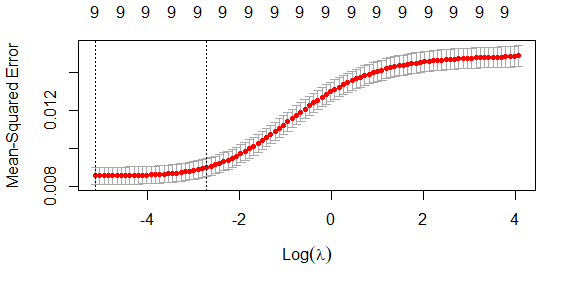
\includegraphics{"images/ridge.png"} \label{ridge}

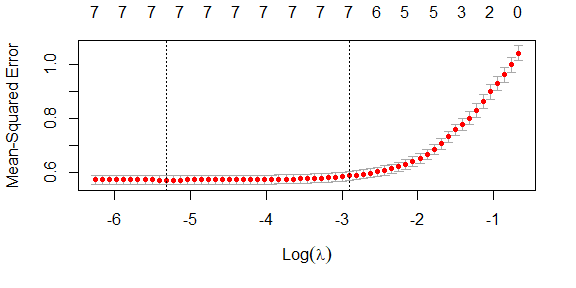
\includegraphics{"images/lasso.png"} \label{lasso}

If we wanted to compare all 6 models visually we could look at the bar
graph below .

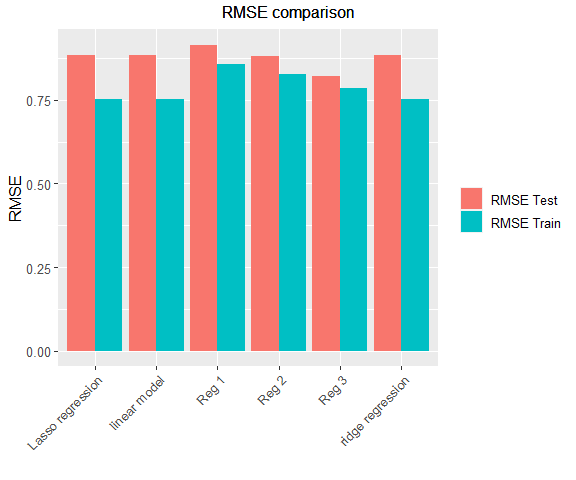
\includegraphics{"images/RMSE.png"} \label{RMSEimg}

\hypertarget{predicting-race}{%
\subsection{\texorpdfstring{Predicting Race
\label{race}}{Predicting Race }}\label{predicting-race}}

\begin{figure}
\centering
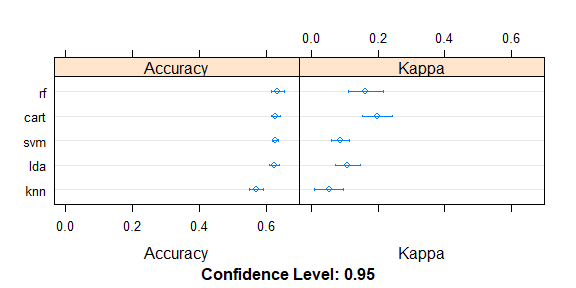
\includegraphics{"images/unbal.png"}
\caption{Machine Learning applied to unbalanced data}
\end{figure}

\begin{figure}
\centering
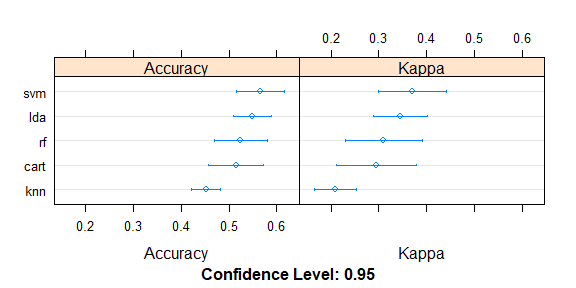
\includegraphics{"images/bal1.png"}
\caption{Machine Learning applied to balanced (undersampled) data}
\end{figure}

\begin{figure}
\centering
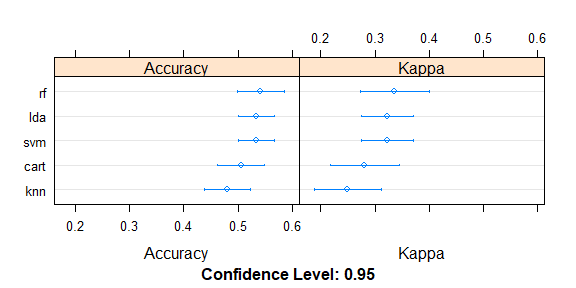
\includegraphics{"images/bal2.png"}
\caption{Machine Learning applied to balanced data}
\end{figure}

The graph below displays the confusion matrix and the tables report the
relevant statistics.

\begin{figure}
\centering
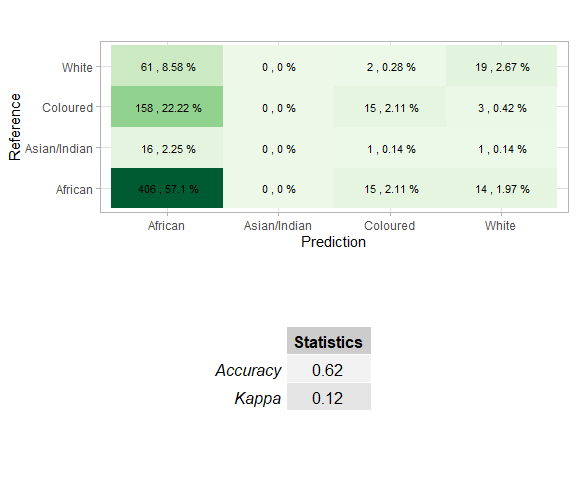
\includegraphics{"images/cmrf.png"}
\caption{Random Forest Confusion Matrix}
\end{figure}

\begin{figure}
\centering
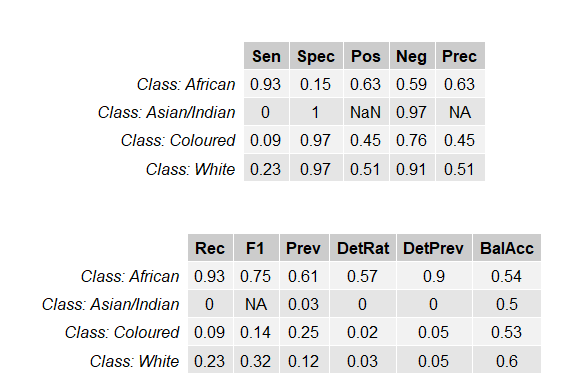
\includegraphics{"images/statsrf.png"}
\caption{Random Forest Statistics}
\end{figure}

\hypertarget{conclusion}{%
\section{Conclusion}\label{conclusion}}

\newpage

\hypertarget{references}{%
\section*{References}\label{references}}
\addcontentsline{toc}{section}{References}

\hypertarget{refs}{}
\begin{CSLReferences}{1}{0}
\leavevmode\hypertarget{ref-k}{}%
Kassambara, A. 2018a. Cross-validation essentials in r.

\leavevmode\hypertarget{ref-rmse}{}%
Kassambara, A. 2018b. Linear regression essentials in r. {[}Online{]},
Available:
\url{http://www.sthda.com/english/articles/40-regression-analysis/165-linear-regression-essentials-in-r/}.

\leavevmode\hypertarget{ref-Texevier}{}%
Katzke, N.F. 2017. \emph{{Texevier}: {P}ackage to create elsevier
templates for rmarkdown}. Stellenbosch, South Africa: Bureau for
Economic Research.

\leavevmode\hypertarget{ref-nids}{}%
\emph{National income dynamics study 2017, wave 5 dataset}. 2018. Cape
Town, South Africa: Department of Planning, Monitoring,; Evaluation
{[}funding agency{]} \& DataFirst {[}distributor{]}. {[}Online{]},
Available: \url{https://doi.org/10.25828/fw3h-v708}.

\leavevmode\hypertarget{ref-kfold}{}%
Rodriguez, J.D., Perez, A. \& Lozano, J.A. 2009. Sensitivity analysis of
k-fold cross validation in prediction error estimation. \emph{IEEE
transactions on pattern analysis and machine intelligence}.
32(3):569--575.

\leavevmode\hypertarget{ref-econ}{}%
Studenmund, A.H. 2014. \emph{Using econometrics a practical guide}.
Pearson.

\end{CSLReferences}

\hypertarget{appendix}{%
\section*{Appendix}\label{appendix}}
\addcontentsline{toc}{section}{Appendix}

\hypertarget{appendix-a}{%
\subsection*{Appendix A}\label{appendix-a}}
\addcontentsline{toc}{subsection}{Appendix A}

Some appendix information here

\hypertarget{appendix-b}{%
\subsection*{Appendix B}\label{appendix-b}}
\addcontentsline{toc}{subsection}{Appendix B}

\bibliography{Tex/ref}





\end{document}
